\section{Sample-Level Decomposition for the Image-Classification Results}
\label{appendix:sample-level}

The image-classification results also report a sample-level decomposition.
For those results and this appendix, index mini-batches by $t=0,\ldots,T-1$,
write their size as $m$, and let $g_i^{(t)}$ be the gradient of sample $i$
evaluated at $\theta_t$. The batch mean is
\[
  G_{B_t}:=\frac{1}{m}\sum_{i=1}^m g_i^{(t)}.
\]
Thus, $G_{B_t}$ in this indexing is $g_{t+1}$ in
Section~\ref{sec:displacement}. For constant-step plain SGD,
\begin{equation}
  \theta_T=\theta_0-\eta\sum_{t=0}^{T-1}G_{B_t}.
  \label{eq:final_theta_expression}
\end{equation}
Taking the squared norm gives
\begin{equation}
\begin{aligned}
\|\theta_T\|^2={}&\|\theta_0\|^2
 -2\eta\sum_{t=0}^{T-1}\theta_0^\top G_{B_t}\\
 &+\eta^2\Bigl\|\sum_{t=0}^{T-1}G_{B_t}\Bigr\|^2.
\end{aligned}
\label{eq:norm_split_terms}
\end{equation}
Define the initialization--trajectory term
$C:=-2\eta\sum_{t=0}^{T-1}\theta_0^\top G_{B_t}$ and the sample-level sums
\begin{equation}
\begin{aligned}
S_1&:=\sum_{t=0}^{T-1}\sum_{i=1}^m\|g_i^{(t)}\|^2,\\
S_2&:=\sum_{t=0}^{T-1}\sum_{i=1}^m
       \sum_{\substack{j=1\\j\ne i}}^m g_i^{(t)\top}g_j^{(t)},\\
S_3&:=2\sum_{t=0}^{T-1}\sum_{u=0}^{t-1}
       \sum_{i,j=1}^m g_i^{(t)\top}g_j^{(u)}.
\end{aligned}
\label{eq:s_def}
\end{equation}
The sums collect per-sample energy, within-batch interactions, and all
cross-step interactions, respectively. Their expansion gives the exact identity
\begin{equation}
\begin{aligned}
\|\theta_T\|^2={}&\|\theta_0\|^2+C\\
 &+\frac{\eta^2}{m^2}(S_1+S_2+S_3).
\end{aligned}
\label{eq:thetaT_full}
\end{equation}
In particular, $(S_1+S_2)/m^2=\sum_t\|G_{B_t}\|^2$ is the batch-gradient
energy, while $S_3/m^2$ is the complete temporal interaction. The latter
cannot generally be recovered from consecutive cosine alone. These identities
specify the quantities displayed in Fig.~\ref{fig:traj_decomp}; they do not
identify their signs with loss reduction or a stability guarantee.

\begin{figure*}[h]
    \centering
    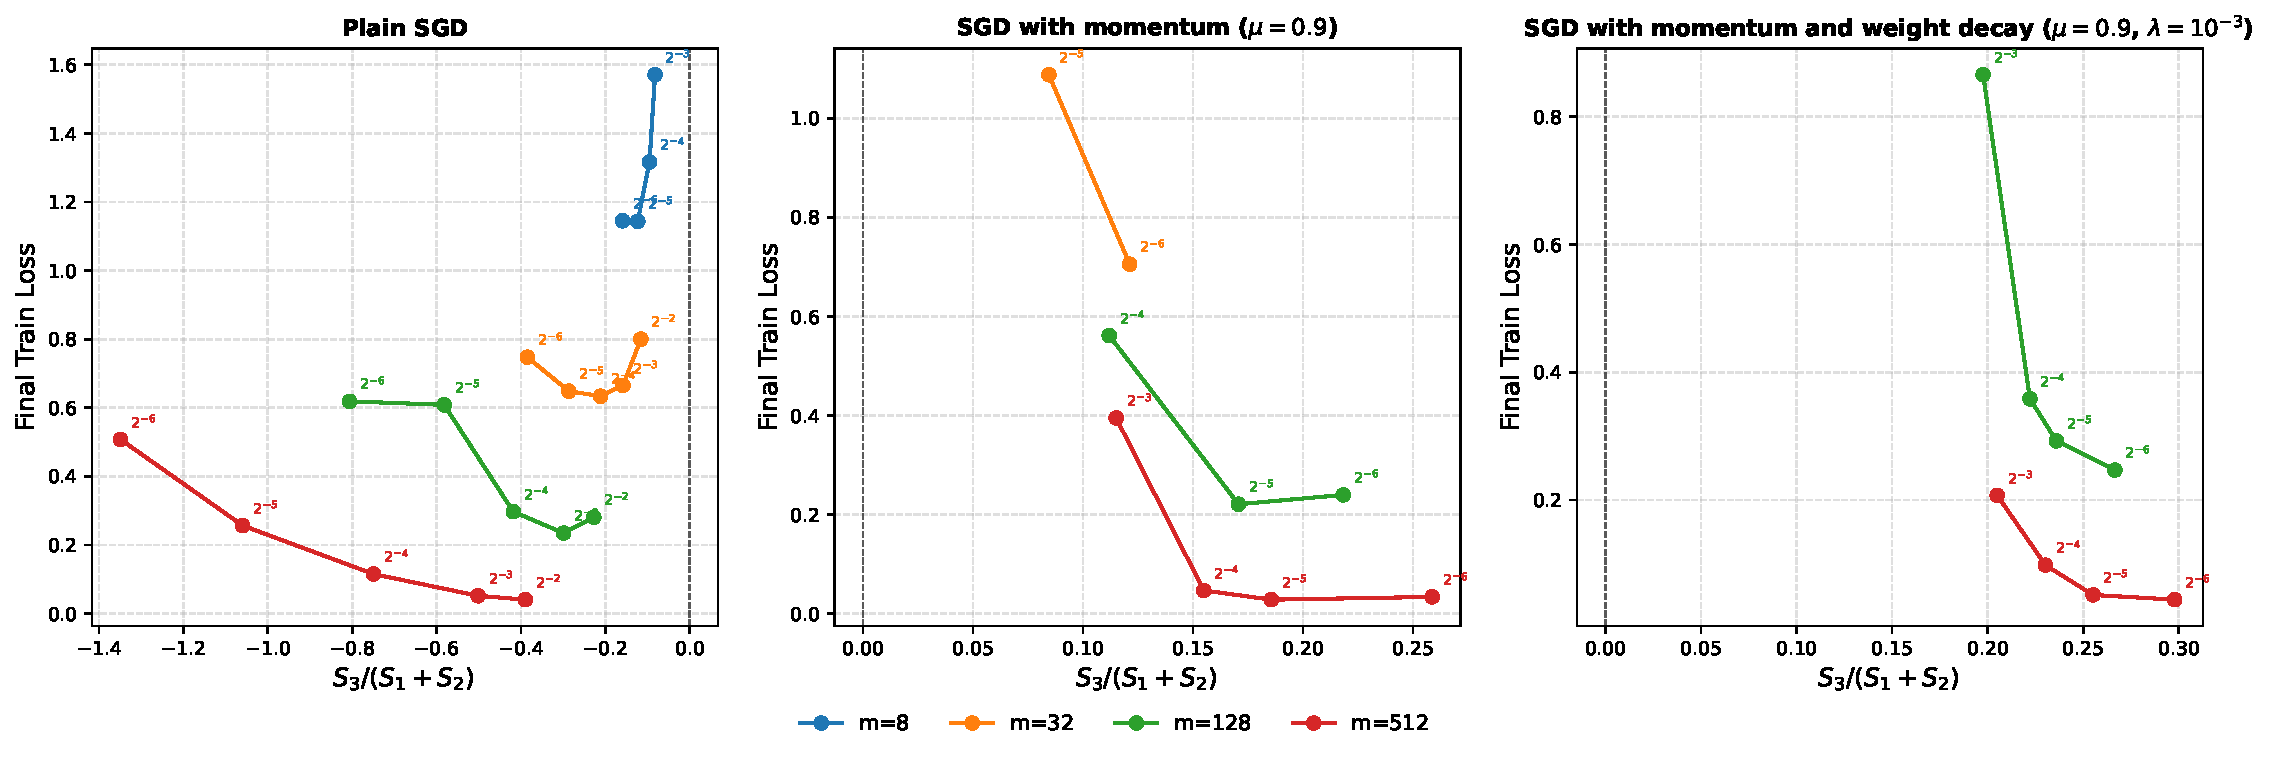
\includegraphics[width=1\linewidth]{figures/interf_ratio_to_loss.pdf}
    \caption{
Final training loss versus the normalized cross-step term \(S_3/(S_1+S_2)\) for VGG in CIFAR-10 with plain SGD (left), SGD with momentum \((\mu=0.9)\) (middle), and SGD with momentum plus weight decay \((\mu=0.9,\lambda=10^{-3})\) (right). Colors indicate batch size \(m\in\{8,32,128,512\}\); markers are annotated with the learning rate \(\{2^{-6}, ..., 2^{-2}\}\). The dashed vertical line denotes the boundary \(S_3=0\).
}
\label{fig:traj_decomp}
\end{figure*}
